%KASCADE gamma search

\section{KASCADE high-energy \texorpdfstring{$\gamma$}{gamma}-ray search}

\begin{frame}{High-energy $\gamma$-ray sources in KASCADE field of view}
  KASCADE data: Efficiency of registration, exposure map *
\end{frame}

\begin{frame}{Diffuse $\gamma$ flux upper-limit based on KASCADE data}
  Upper limit on diffuse gamma flux (by Donghwa) +
\end{frame}

\begin{frame}{$\gamma$-proton separation}
\small
% \begin{figure}[h]
\vspace{-1em}
\begin{center}
    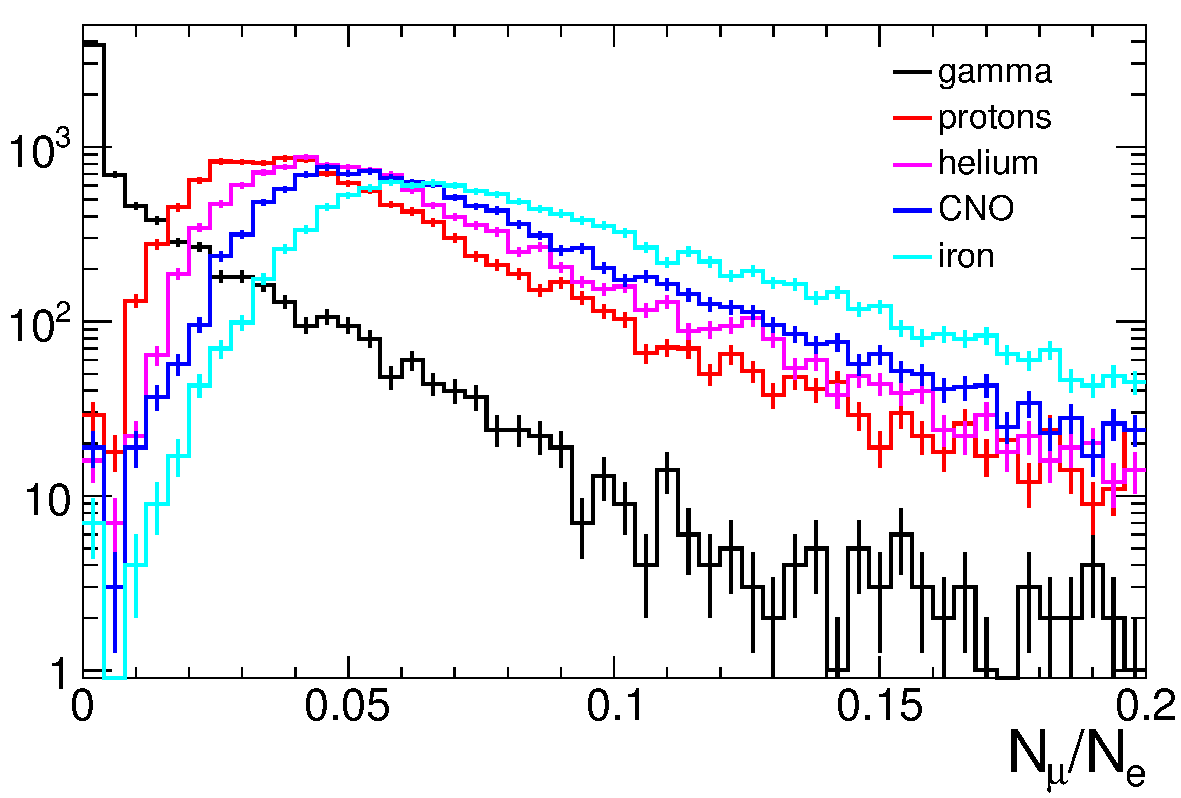
\includegraphics[width=0.65\textwidth]{pics/Nmu_Ne.pdf}
    
    Distribution of $N_\mu / N_e$ for various primary CR components.
\end{center}
%   Распределение компонент ливня в зависимости от соотношения мюоной и электронной компоненты ливня
% \caption{
% \vspace{1em}
% }
%  \end{figure}
Taking into account this distribution and the flux upper-limit mentioned above we can make the 
$N_\mu/N_e \in [0, 0.008)$ cut to discriminate $\gamma$ component with ... C.L.
\end{frame}

\begin{frame}{KASCADE statistics estimation for $2HWC_J2013+415$}
There supposed to be 3 slides on this
%  Оценка количества событий вокруг 2HWC_J2013+415 +-
\end{frame}
